%%%%%%%%%%%%%%%%%%%%%%%%%%%%%%%%%%%%%%%%%
% Short Sectioned Assignment LaTeX Template Version 1.0 (5/5/12)
% This template has been downloaded from: http://www.LaTeXTemplates.com
% Original author:  Frits Wenneker (http://www.howtotex.com)
% License: CC BY-NC-SA 3.0 (http://creativecommons.org/licenses/by-nc-sa/3.0/)
%%%%%%%%%%%%%%%%%%%%%%%%%%%%%%%%%%%%%%%%%

% \documentclass[paper=a4, fontsize=11pt]{scrartcl} % A4 paper and 11pt font size
\documentclass[11pt, a4paper]{book}
\usepackage[T1]{fontenc} % Use 8-bit encoding that has 256 glyphs
\usepackage[utf8]{inputenc}
\usepackage{fourier} % Use the Adobe Utopia font for the document - comment this line to return to the LaTeX default
\usepackage{listings} % para insertar código con formato similar al editor
\usepackage[spanish, es-tabla]{babel} % Selecciona el español para palabras introducidas automáticamente, p.ej. "septiembre" en la fecha y especifica que se use la palabra Tabla en vez de Cuadro
\usepackage{url} % ,href} %para incluir URLs e hipervínculos dentro del texto (aunque hay que instalar href)
\usepackage{graphics,graphicx, float} %para incluir imágenes y colocarlas
\usepackage[gen]{eurosym} %para incluir el símbolo del euro
\usepackage{cite} %para incluir citas del archivo <nombre>.bib
\usepackage{enumerate}
\usepackage{hyperref}
\usepackage{graphicx}
\usepackage{tabularx}
\usepackage{booktabs}

\usepackage[table,xcdraw]{xcolor}
\hypersetup{
	colorlinks=true,	% false: boxed links; true: colored links
	linkcolor=black,	% color of internal links
	urlcolor=cyan		% color of external links
}
\renewcommand{\familydefault}{\sfdefault}
\usepackage{fancyhdr} % Custom headers and footers
\pagestyle{fancyplain} % Makes all pages in the document conform to the custom headers and footers
\fancyhead[L]{} % Empty left header
\fancyhead[C]{} % Empty center header
\fancyhead[R]{Miguel Ángel Martín Rodríguez} % My name
\fancyfoot[L]{} % Empty left footer
\fancyfoot[C]{} % Empty center footer
\fancyfoot[R]{\thepage} % Page numbering for right footer
%\renewcommand{\headrulewidth}{0pt} % Remove header underlines
\renewcommand{\footrulewidth}{0pt} % Remove footer underlines
\setlength{\headheight}{13.6pt} % Customize the height of the header

\usepackage{titlesec, blindtext, color}
\definecolor{gray75}{gray}{0.75}
\newcommand{\hsp}{\hspace{20pt}}
\titleformat{\chapter}[hang]{\Huge\bfseries}{\thechapter\hsp\textcolor{gray75}{|}\hsp}{0pt}{\Huge\bfseries}
\setcounter{secnumdepth}{4}
\usepackage[Lenny]{fncychap}


\begin{document}

	% Plantilla portada UGR
	\begin{titlepage}
\newlength{\centeroffset}
\setlength{\centeroffset}{-0.5\oddsidemargin}
\addtolength{\centeroffset}{0.5\evensidemargin}
\thispagestyle{empty}

\noindent\hspace*{\centeroffset}\begin{minipage}{\textwidth}

\centering

\includegraphics[width=0.9\textwidth]{logos/logo_ugr.jpg}\\[1.4cm]

\textsc{ \Large TRABAJO FIN DE GRADO\\[0.2cm]}
\textsc{ GRADO EN INGENIERIA INFORMATICA}\\[1cm]

{\Huge\bfseries Título \\}
\noindent\rule[-1ex]{\textwidth}{3pt}\\[3.5ex]
{\large\bfseries Subtítulo }
\end{minipage}

\vspace{2.5cm}
\noindent\hspace*{\centeroffset}
\begin{minipage}{\textwidth}
\centering

\textbf{Autor}\\ {Estudiante}\\[2.5ex]
\textbf{Director}\\ {Tutor(a)(es)}\\[2cm]

\includegraphics[width=0.3\textwidth]{logos/etsiit_logo.png}\\[0.1cm]
\textsc{Escuela Técnica Superior de Ingenierías Informática y de Telecomunicación}\\
\textsc{---}\\
Granada, Junio de 201x
\end{minipage}
\end{titlepage}


	% Plantilla prefacio UGR
	\thispagestyle{empty}

\begin{center}
{\large\bfseries Título \\ Subtítulo }\\
\end{center}
\begin{center}
Nombre Del Estudiante\\
\end{center}

%\vspace{0.7cm}

\vspace{0.5cm}
\noindent\textbf{Palabras clave}: \textit{software libre}
\vspace{0.7cm}

\noindent\textbf{Resumen}\\
	

\cleardoublepage

\begin{center}
	{\large\bfseries Same, but in English}\\
\end{center}
\begin{center}
	Student's name\\
\end{center}
\vspace{0.5cm}
\noindent\textbf{Keywords}: \textit{open source}, \textit{floss}
\vspace{0.7cm}

\noindent\textbf{Abstract}\\


\cleardoublepage

\thispagestyle{empty}

\noindent\rule[-1ex]{\textwidth}{2pt}\\[4.5ex]

D. \textbf{Tutora/e(s)}, Profesor(a) del ...

\vspace{0.5cm}

\textbf{Informo:}

\vspace{0.5cm}

Que el presente trabajo, titulado \textit{\textbf{Chief}},
ha sido realizado bajo mi supervisión por \textbf{Estudiante}, y autorizo la defensa de dicho trabajo ante el tribunal
que corresponda.

\vspace{0.5cm}

Y para que conste, expiden y firman el presente informe en Granada a Junio de 2018.

\vspace{1cm}

\textbf{El/la director(a)/es: }

\vspace{5cm}

\noindent \textbf{(nombre completo tutor/a/es)}

\chapter*{Agradecimientos}






	% Índice de contenidos
	\newpage
	\tableofcontents

	% Índice de imágenes y tablas
	\newpage
	\listoffigures

	% Si hay suficientes se incluirá dicho índice
	\listoftables 
	\newpage

	% Introducción 
	\chapter{Introducción}

Este proyecto es software libre, y está liberado con la licencia \cite{gplv3}.\\

Puede encontrarse en el siguiente repositorio:
\url{https://github.com/migueorg/One-touch-music-streaming-TFG-ETSIIT/}, en el
cual se ha desarrollado desde el principio en abierto.

\section{Descripción del problema}
En los tiempos en los que estamos, cada vez es más normal escuchar música o
podcasts de fondo mientras hacemos otras tareas de nuestro día a día. Escuchamos
contenido mientras trabajamos, vamos en el coche, de camino al trabajo, de
vuelta a casa, mientras cocinamos, limpiamos, hay quienes también escuchan algún
tipo de podcast, ruido blanco o sonido para irse a dormir, entre muchos otros
más escenarios. 

A su vez, en el contexto informático en el que estamos, también le hemos dado la
espalda a los cables siempre que nos sea posible. Los auriculares inalámbricos
son un obligatorio en el día a día de muchas personas, facilitando así la
integración de la música en cada vez más contextos diferentes de nuestra vida.
Sin embargo, aún teniendo en cuenta los avances en el campo del \emph{IoT}, no
es tan fácil mantener esa sensación de integración y continuidad respecto a la
escucha de música. Ya que si queremos seguir escuchando en algún altavoz
inteligente la misma canción o podcast que veníamos escuchando en el móvil,
tendremos que empezar a interactuar con menús, dictar comandos (que no siempre
funcionan) al asistente virtual; o alguna otra alternativa compleja o cara.\\

\section{Motivación}
Por tanto, una vez puestos en contexto, la motivación de este proyecto es la de
poder brindar dicha sensación de continuidad con un ecosistema abierto, tanto
para el móvil emisor como para el altavoz receptor. Esto hará que el coste para
disfrutar de dicha funcionalidad sea notablemente más bajo que la vía existente
actual usando el ecosistema de \emph{Apple}. Este coste limitará la versión
mínima del \emph{JDK} de \emph{Android} que se utilizará para el proyecto en
basándonos en el coste de dispositivos compatibles y funciones requeridas para
llevar a cabo la funcionalidad.

Así mismo, este proyecto mantiene como principales objetivos (entre otros que se
comentarán con más detalle a continuación) la facilidad de utilización,
simpleza, accesibilidad y funcionamiento automático e independiente; atributos
que la actual solución comercial posee.

Esto se hará creando un servicio dotado por un emisor y un receptor de audio, el
cual sea capaz de enviar el sonido a dicho receptor. En el receptor se podrá
conectar altavoces de un tercero, ya sea por cable, jack, \emph{Bluetooth} o
cualquier vía que sea compatible con el dispositivo en donde se instale el
receptor.

\section{Objetivos}
\begin{itemize}
    \item Se deberá poder transmitir o mandar el sonido que se esté
    reproduciendo en el dispositivo móvil hasta el dispositivo que haga de
    altavoz o receptor.
    \item La comunicación entre ambos dispositivos (móvil y altavoz) deberá de
    llevarse a cabo en menos de 3 segundos para poder mantener la sensación de
    continuidad de la que hemos hablado antes. Más de 3 segundos puede hacer
    creer al usuario que el servicio no está funcionando.
    \item Facilidad de uso y sencillez a la hora de compartir el contenido del
    reproductor al altavoz. El proceso de envío de sonido desde el Android hasta
    el altavoz ha de poder realizarse sin interactuar con menús.
\end{itemize}

\section{Personajes y viajes de usuario}
Los personajes que tienen el problema presentado anteriormente y que, por tanto,
son los que usarán la aplicación para solventarlo son:
\begin{itemize}
    \item Miguel, 52 años, es un contable al que le gusta la tecnología y tiene
    su casa llena de ordenadores viejos, equipos de música antiguos, altavoces,
    etc. Se ha ido adaptando a los cambios de la tecnología con los años, y como
    tal tiene su casa llena de altavoces inteligentes de los que se
    comercializan a día de hoy; aun así, echa de menos la calidad de los equipos
    de antes. Otro inconveniente que ve es que al tener tantos altavoces
    inteligentes conectados en red, cuando va a enviar el contenido al que tiene
    enfrente tiene que elegir entre una extensa lista en la cual, en ocasiones,
    le cuesta ubicarse; en especial cuando vuelve de trabajar escuchando un
    podcast, el cual desea terminarlo mientras prepara la comida. Sin embargo,
    ese proceso de continuar escuchando su podcast justo por donde iba en un
    altavoz inteligente cuando llega a casa es bastante tosco y molesto, pues le
    requiere tener que navegar entre los menús de compartir contenido y
    seleccionar el altavoz que tiene más cerca entre los tantos de su casa.
    Usando este proyecto Miguel desea poder continuar su escucha en sus antiguos
    (pero mejores) altavoces con solo acercar el móvil al dispositivo que haga
    de receptor.
\end{itemize}



\section{Historias de usuario}
A partir de los personajes y los user story presentados anteriormente, podemos
extraer ciertas funcionalidades del proyecto que el público destino espera
obtener o poder hacer. Estas funcionalidades clave tienen forma de las
siguientes historias de usuario:

\begin{enumerate}
    \item
    \href{https://github.com/migueorg/One-touch-music-streaming-TFG-ETSIIT/issues/10}{HU1}:
    Como usuario que busca la mayor automatización y transparencia con la
    tecnología quiero poder seguir escuchando mi reproducción actual manteniendo
    el mismo momento de escucha sin tener que interactuar con ningún menú al
    enviar hacia mis propios altavoces y equipos viejos, con una inversión baja.
    \item
    \href{https://github.com/migueorg/One-touch-music-streaming-TFG-ETSIIT/issues/14}{HU4}:
    Como persona ajena al proyecto quiero conocer las decisiones que se han
    tomado al desarrollar el proyecto para poder entender por qué se han
    empleado ciertas plataformas y componentes y poder continuar o modificar su
    desarrollo si fuese necesario.
\end{enumerate}

Nótese que además de las funcionalidades que el usuario final espera obtener,
también se ha dedicado una historia de usuario (HU5) que personifica al tribunal o
a cualquier persona que en el futuro encuentre este proyecto y quiera conocer
por qué se ha actuado de la forma que se ha hecho durante todo el trabajo.

\section{Milestones}
Los productos mínimamente viables o \emph{releases} que se irán haciendo durante el
desarrollo se han estimado que serán los siguientes:

\begin{enumerate}
    \item \href{https://github.com/migueorg/One-touch-music-streaming-TFG-ETSIIT/milestone/1}{M0}: Repositorio y documentación funcional sobre la que empezar a programar.
    \item \href{https://github.com/migueorg/One-touch-music-streaming-TFG-ETSIIT/milestone/2}{M1}: Captar el audio del teléfono Android para transmitirlo.
    \item \href{https://github.com/migueorg/One-touch-music-streaming-TFG-ETSIIT/milestone/3}{M2}: Recibir en un dispositivo diferente el audio previamente transmitido.
    \item \href{https://github.com/migueorg/One-touch-music-streaming-TFG-ETSIIT/milestone/4}{M3}: Automatizar la tarea de envío y recepción en un solo gesto/toque
    \item \href{https://github.com/migueorg/One-touch-music-streaming-TFG-ETSIIT/milestone/5}{M4}: Memoria entregable para el tribunal.
    \item \href{https://github.com/migueorg/One-touch-music-streaming-TFG-ETSIIT/milestone/6}{M5}: Presentación.
\end{enumerate}

	% Descripción del problema y hasta donde se llega
	\chapter{Descripción del problema}



	% Estado del arte
	% 	1. Crítica al estado del arte
	% 	2. Propuesta
	\chapter{Estado del arte}

El software libre y sus licencias \cite{gplv3} ha permitido llevar a cabo una expansión del
aprendizaje de la informática sin precedentes.

\section{Análisis de las posibles soluciones al problema propuesto}

Si intentamos solucionar el problema introducido al principio del documento
usando las alternativas existentes actualmente nos vamos a encontrar con
soluciones poco amigables con el usuario, poco eficaces, soluciones de código
privativo y/o demasiado caras.

Usaré el siguiente ejemplo práctico para testear las soluciones actuales y
evaluar el estado del arte: Si llegamos a casa del trabajo, y hemos vuelto
escuchando un podcast en nuestros auriculares inalámbricos mientras andábamos;
al llegar a casa y ponernos a preparar la comida nos gustaría poder seguir
escuchando el podcast por el mismo minuto en el que íbamos pero en los altavoces
de casa. 

\subsection{Solución tradicional}
Para hacer esto, simplemente podríamos conectar el móvil al altavoz mediante el
\emph{jack} de 3.5, sin embargo, los móviles actualmente carecen de dicho puerto
(salvo pocas excepciones). 

\subsection{Solución asistentes de voz}
Otra opción sería emplear cualquiera de los asistentes de voz como lo son
(\emph{Alexa, Google Assistant, Siri}) y pedirle que reproduzca el podcast que
estábamos escuchando, el problema de esto es que tendremos que recordar el
nombre concreto del podcast, tenemos que ponernos a hablarle al asistente lo
cual rompe la sensación de integración y continuidad, y este tiene que ser capaz
de entendernos correctamente, lo cual no pasa siempre. Adicionalmente
requeriríamos de un altavoz inteligente con micrófono activo de cualquiera de las
marcas mencionadas anteriormente, el cual debería incorporar dicho asistente de
voz. 

\subsection{Solución \emph{big tech}}
Otra opción más, la cual es compatible con la mayoría de altavoces con
asistentes integrados, sería la de tener el altavoz en red y mandar el podcast
desde el móvil a través de protocolos como \emph{Google Cast, AirPlay o Spotify
Connect}, lo cual es una de las opciones más rápidas y sencillas, pero implica
tener que estar navegando a través de aplicaciones e interfaces hasta llegar a
la opción de enviar contenido. Y en el caso de que tengamos muchos altavoces en
red, tendremos que elegir de entre una lista amplia de dispositivos, al cual
queremos enviar dicho contenido. De nuevo, este último caso, aún siendo el más
factible, rompe mucho con la sensación de integración y continuidad de la que
hablé anteriormente. 

\subsection{Solución \emph{Apple}} Sin embargo, \emph{Apple} sí que tiene una
solución para esto integrada en su ecosistema. Para los usuarios que tengan un
\emph{iPhone} y un \emph{HomePod} \cite{HomePod}, permiten que la reproducción
del \emph{iPhone} continúe en el \emph{HomePod} simplemente con acercar el
\emph{iPhone} al \emph{HomePod}, sin la necesidad de navegar por interfaces ni
seleccionar nada. Todo de forma transparente para el usuario y en cuestión de
segundos. 

Para ello \emph{Apple} emplea un chip propio llamado \emph{Apple U1} \cite{U1}
en ambos dispositivos (\emph{iPhone} y \emph{HomePod}), el cual es un chip que
dota a los dispositivos de conectividad a través de
\href{https://en.wikipedia.org/wiki/Ultra-wideband}{\emph{UWB (Ultra
Wideband)}}. Este chip trabaja en una radiofrecuencia entre los 6 y 8GHz,
permitiendo así una comunicación de bajo alcance, muy bajo consumo, pero alto
ancho de banda a partir de los estándares
\href{https://es.wikipedia.org/wiki/IEEE_802.15#Grupo_de_trabajo_4_(WPAN_de_baja_velocidad)}{IEEE
802.15.4a y IEEE 802.15.4z}, y es usado para determinar una precisión espacial
entre los dispositivos que la porten. Gracias a esto, tanto \emph{iPhone} como
\emph{HomePod} saben que están apuntándose el uno al otro, para, acto seguido
mediante \emph{Apple Handoff} \cite{Handoff} comunicarse a través de
\emph{bluetooth} y \emph{wifi}, y de esta forma conocer la canción que se estaba
reproduciendo en el \emph{iPhone} y compartir la reproducción a través de
\emph{AirPlay} \cite{AirPlay}.

El problema de esta solución es que no es de código abierto, en la que además se usan
tecnologías propias inaccesibles para cualquier usuario ajeno al ecosistema de Apple.

\section{Conclusión tras estudiar el mercado}
Tras repasar todas las posibilidades existentes para solventar el problema
actualmente, vemos que la solución más elegante es la que tiene \emph{Apple}. El
problema es que esa solución es de código privativo, además de estar en un
ecosistema muy cerrado, siendo exclusiva de algunos dispositivos \emph{Apple}.
Si queremos disfrutar de la automatización y transparencia que se aprecia en
esta solución no encontramos nada similar ni cercano. Es por eso que nace la
necesidad de crear este proyecto, persiguiendo un resultado similar al que
proporciona \emph{Apple}, pero enfocado en dispositivos \emph{Android} con
tecnologías más comunes y baratas.

	
	\chapter{Planificación}

La planificación es algo esencial para todos los proyectos, y juega un papel aún 
más importante si cabe, cuando se involucra el desarrollo ágil, como es el caso. 

Por tanto, en este capítulo detallaremos que metodologías se van a seguir, como 
se va a organizar temporalmente el proyecto, y como se ha ido siguiendo el 
desarrollo y asegurando la calidad del mismo. 

\section{Metodología utilizada}

A continuación documentaremos que herramientas y métodos se ha ido empleando 
durante el proyecto para ir guiando su desarrollo. Asegurando de esta forma, que 
con el tiempo no se pierda el enfoque y los objetivos iniciales. 

\subsection{Control de versiones}

La metodología que ha servido de motor principal sobre el que desarrollar este
proyecto ha sido \emph{Git}. Gracias a esto, no solo hemos podido llevar un
histórico detallado para el código y documentación durante todo el desarrollo,
sino que hemos podido aprovechar sus múltiples herramientas como las
\emph{branches}, \emph{pull request}, etc. para agilizar el proyecto. Así mismo,
\emph{GitHub} ha sido el alojamiento para este proyecto.

\begin{figure}[H]
    \centering
    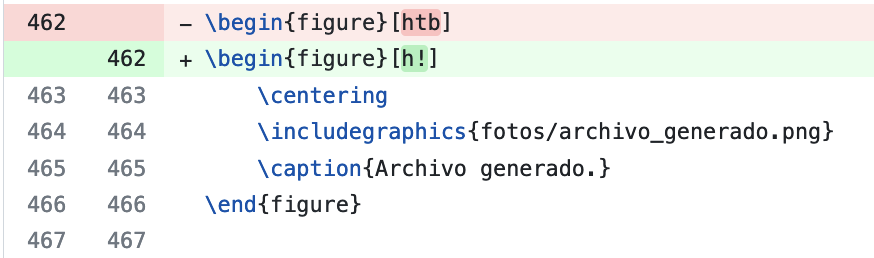
\includegraphics[width=0.5\textwidth]{fotos/control_versiones.png}
    \caption{Muestra de histórico de cambios.}
\end{figure}

\subsection{Kanban}

\emph{Kanban} es una metodología para organizar equipos, con la que representar
de manera gráfica los flujos y la carga de trabajo. Así pues con un simple
vistazo se puede comprobar que hay pendiente por hacer, en que se está
trabajando actualmente y que es lo que se lleva hecho. \emph{GitHub} cuenta con
la posibilidad de incorporar una (y varias) \emph{Kanban} a un repositorio, bajo
el apartado \emph{projects} del mismo, la cual se vaya actualizando con los
\emph{issues, commits, pull request, etc.}

Por esto, se ha utilizado una \emph{Kanban} en el desarrollo de este proyecto:

\begin{figure}[H]
    \centering
    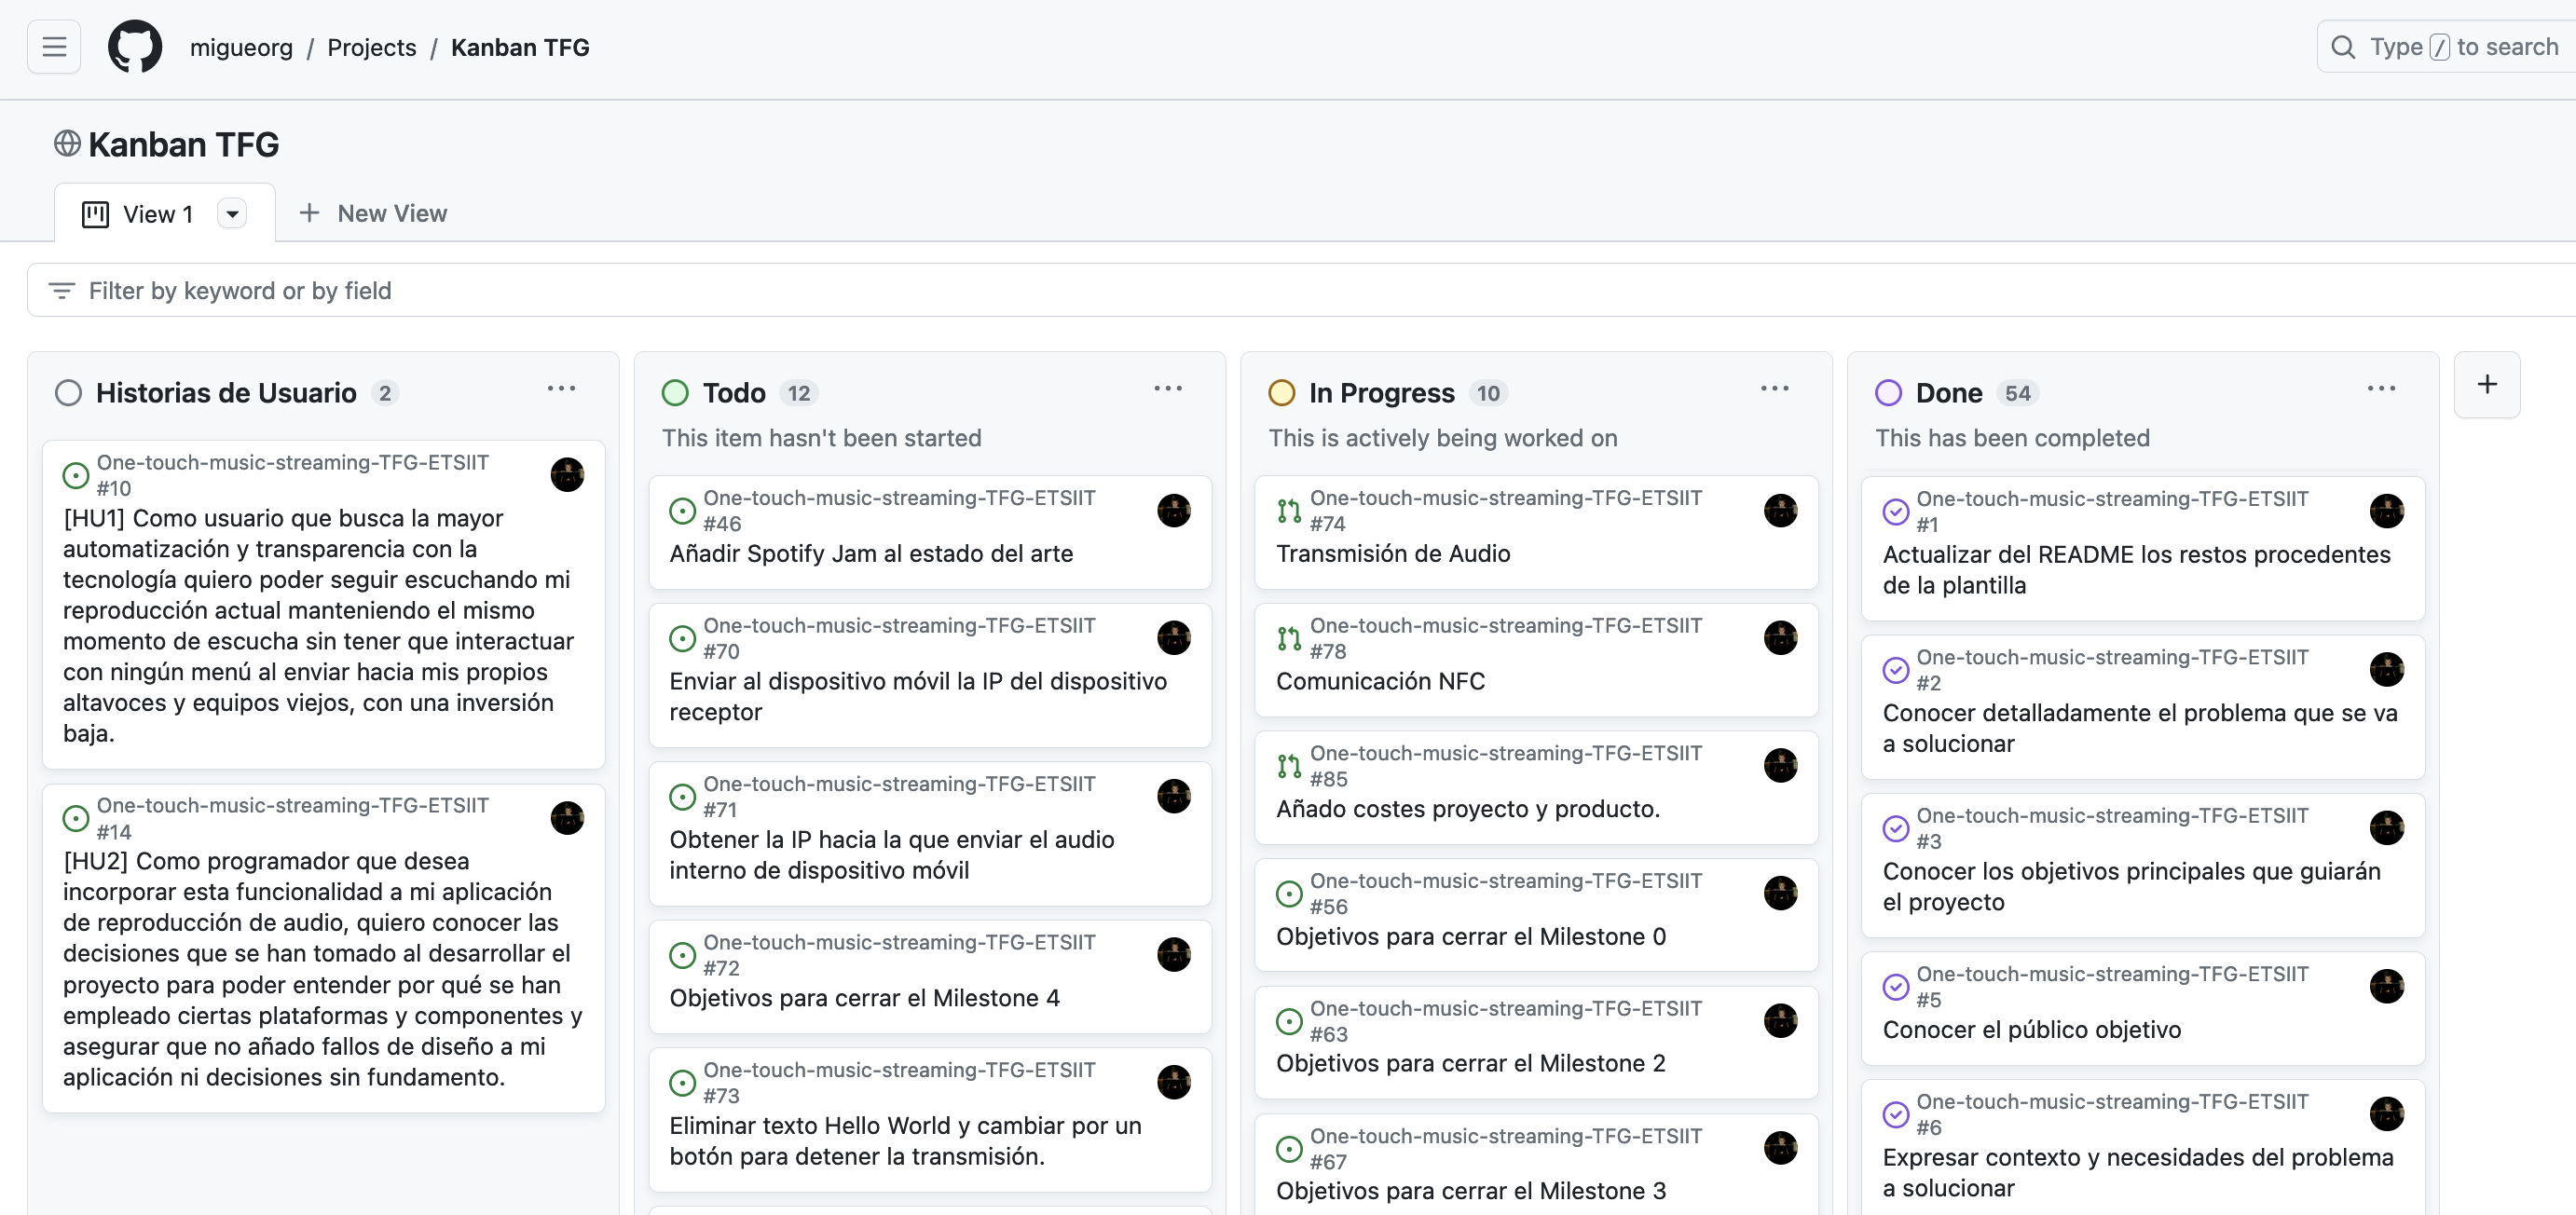
\includegraphics[width=\textwidth]{fotos/kanban.png}
    \caption{Kanban del proyecto.}
\end{figure}

\subsection{Issues}

A través de los propios \emph{issues} de \emph{GitHub} se ha ido seguimiento de
las tareas a realizar, así como los \emph{bugs} o posibles mejoras pendientes.
Durante el desarrollo, todos los \emph{commits} han ido referenciando a un
\emph{issue}, al igual que todos los \emph{commits} han sido los encargados de cerrar
todos los \emph{issues} cuando la tarea estaba finalizada. Además, las
\hyperref[historias-usuario]{historias de usuario de las que hablamos en el
capítulo de introducción} han sido representadas en forma de issue.

\begin{figure}[H]
    \centering
    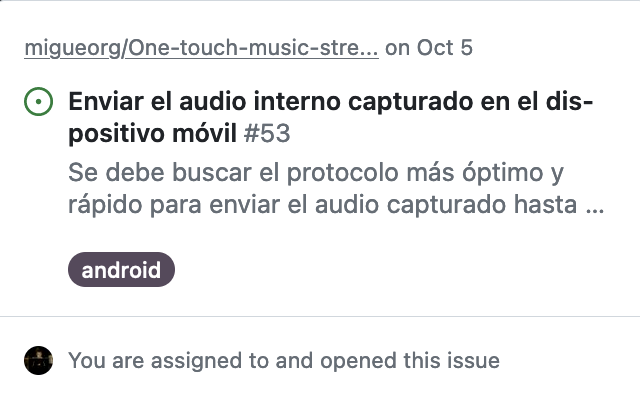
\includegraphics[width=0.5\textwidth]{fotos/issues.png}
    \caption{Ejemplo de issue del proyecto.}
\end{figure}

\subsection{Pull request}

Cada proceso de añadir cualquier elemento al proyecto, primero ha pasado por un
\emph{pull request}; de este método, se ha podido llevar un control y revisión
exhausto de absolutamente todo lo que se ha añadido al mismo, por mínima
funcionalidad, o cambio que fuese. Detallando en el propio \emph{pull request}
que commit (y por tanto parte de que \emph{issue}) modificaba cada línea.

\begin{figure}[H]
    \centering
    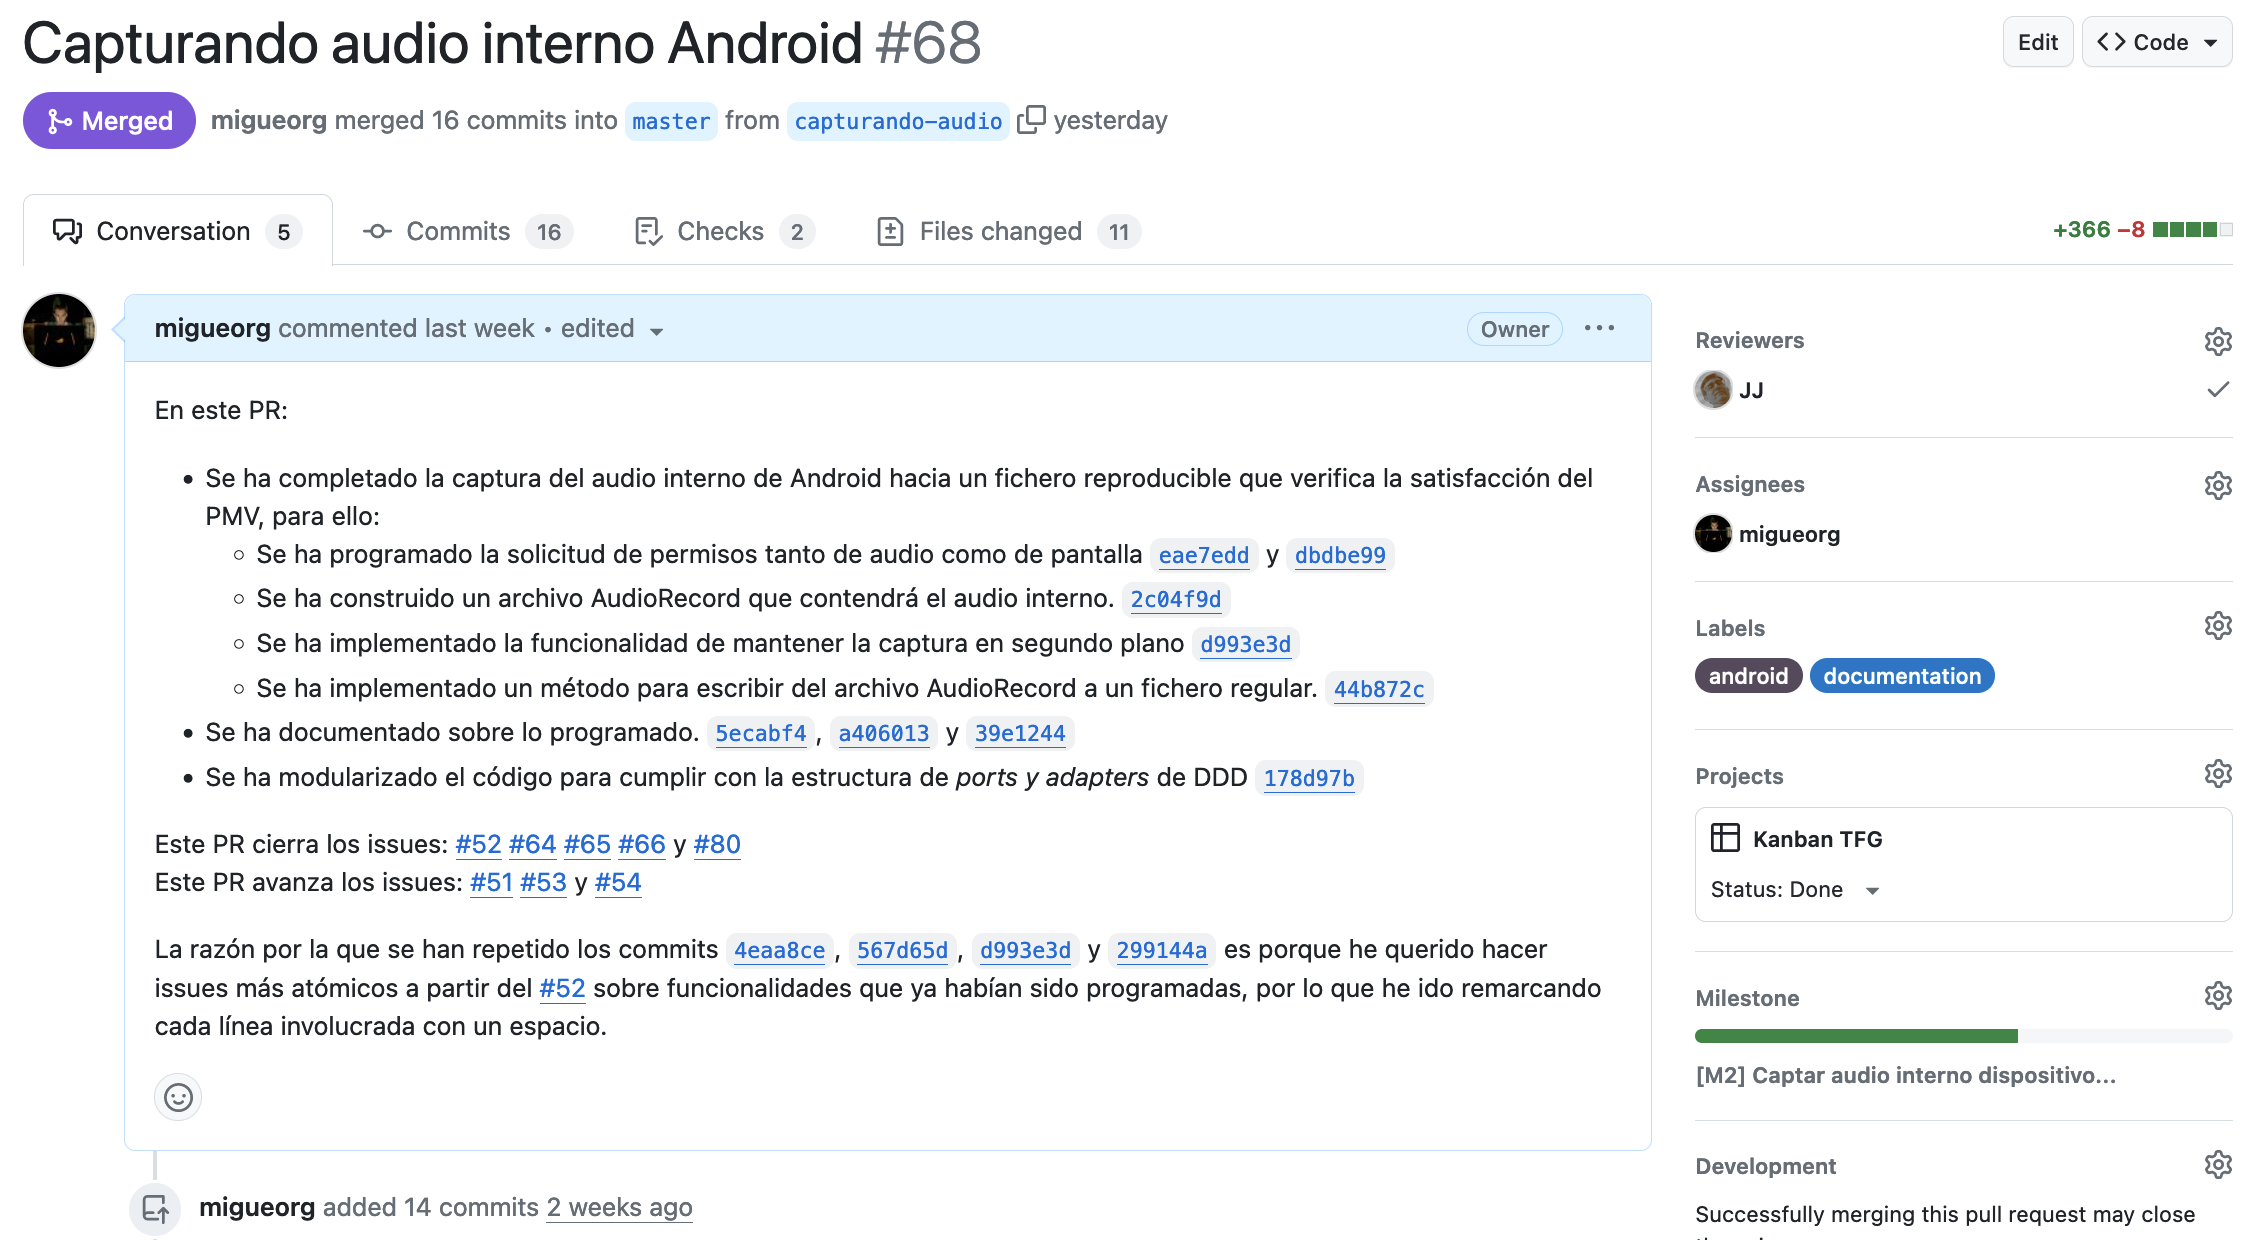
\includegraphics[width=0.8\textwidth]{fotos/pull_request.png}
    \caption{Pull request ya aceptada y fusionada.}
\end{figure}


\section{Asegurando y verificando la calidad}

\subsection{Corrector ortográfico}
Para poder asegurar la calidad que buscamos siguiendo los principios del manifiesto
ágil \cite{agile-manifiesto}, no solo del código, sino también del documento
entregable en cuanto a calidad gramatical y ortográfica se refiere, se ha
implementado un corrector que verificará en todo momento que cualquier adición a
la documentación está libre de faltas. 

Para elegir dicho corrector entre todas las posibles alternativas que existen de 
la misma, se ha seguido un proceso de selección en el cual se establecerán 
inicialmente unos criterios de búsqueda con el que encontrar las herramientas. 
Posteriormente, se evaluarán todas las herramientas encontradas usando los 
criterios de selección previamente establecidos.: 

\subsubsection{Criterios de búsqueda}

Los criterios a través de los cuales buscaremos los candidatos para
posteriormente evaluar si cumplen los requisitos de selección:
\begin{itemize}
    \item Deben de incluir el idioma español. No todos los \emph{spell checkers}
    incluyen el idioma español, y si lo incluyen suelen ser de manera muy
    limitada y no tan completa como el idioma base en el que fueron programados.
    \item Deben poderse añadir como \emph{GitHub Action} al repositorio para así
    integrarlos en forma de test, y solamente pase si el texto está correcto.
    \item Debe ser compatible con LaTeX.
\end{itemize}

\subsubsection{Criterios de selección}

Los criterios bajo los cuales evaluaremos los candidatos encontrados en la
búsqueda anterior para finalmente seleccionar uno son:
\begin{itemize}
    \item Debe tener una comunidad activa por si es necesario hacer alguna
    pregunta o consulta en el futuro.
    \item Los informes sobre los fallos existentes deben ser lo más legible y
    fácil de entender posible.
    \item Se valorará que ofrezca posibles correcciones.
    \item Se valorará la posibilidad de excluir palabras del análisis. 

\end{itemize}


\subsubsection{Opciones encontradas según los criterios de búsqueda establecidos}

Tras buscar \emph{spell checkers} que cumplan los requisitos de búsqueda son:

\begin{itemize}
    \item \href{https://github.com/marketplace/actions/textidote-action}{TeXtidote Action}
\end{itemize}

Desafortunadamente, únicamente he podido encontrar un \emph{spell checker} que
cumpliese todos los requisitos de búsqueda previamente establecidos. Ya que otros
encontrados \textbf{no cumplían algunos de los requisitos}:
\begin{itemize}
    \item \href{https://github.com/marketplace/actions/cspell-action}{cspell-action} Pensado principalmente para código no para documentos LaTeX. Nada de español.
    \item \href{https://github.com/marketplace/actions/spell-checker-action}{Spell Checker Action}: Compatible únicamente con inglés. No está centrado en LaTeX. 
    \item \href{https://github.com/valentjn/vscode-ltex}{VSCode LTeX}: No dispone de GitHub Action.
    \item \href{https://github.com/erodner/latex-checks}{LaTeX-Checks}: No dispone de GitHub Action. Solo para inglés y alemán.
\end{itemize}

\subsubsection{Proceso de selección y estudio}
Dado que solo hay un corrector ortográfico a analizar, el proceso de estudio y
decisión entre las alternativas no es estrictamente necesario, pero igualmente
se realizará según los criterios de selección previamente establecidos para ver
en que lugar queda: 

\begin{todolist}
    \item[\xcmark] Debe tener una comunidad activa por si es necesario hacer
    alguna pregunta o consulta en el futuro. Cumple este requisito pues se
    mantiene activo en GitHub resolviendo los \emph{issues} y \emph{PR} de la
    comunidad.
    \item[\xcmark] Los informes sobre los fallos existentes deben ser lo más
    legible y fácil de entender posible. Cumple este requisito pues genera un
    reporte en \emph{HTML} con los problemas resaltados en colores llamativos.
    \item[\xcmark] Se valorará que ofrezca posibles correcciones. Cumple este
    requisito pues en dicho reporte al poner el cursor encima te sugiere
    revisiones.
    \item[\xcmark] Se valorará la posibilidad de excluir palabras del análisis.
    Cumple el requisito aunque bastante raspado, ya que permite excluir palabras
    mediante un diccionario de palabras excluidas, sin embargo, no permite
    excluir una única aparición puntual de la misma.
\end{todolist}

\subsubsection{Conclusión}
Finalmente, dado que es la única alternativa que se ajusta completamente a los
requisitos de búsqueda y además cumple en mayor o menor medida con los
requisitos de selección establecidos, se ha implementado esta solución como
\emph{GitHub Action} en el repositorio, para asegurar la calidad del documento
entregable.

\subsection{Test runner: Java y Kotlin}

\subsubsection{Criterios de búsqueda}

Los criterios a través de los cuales buscaremos los candidatos para
posteriormente evaluar si cumplen los requisitos de selección:
\begin{itemize}
    \item Se buscarán test runners que sean compatibles con Java y Kotlin.
    Puesto que vamos a trabajar con dos lenguajes distintos, pero que a su vez
    comparten muchas similitudes y bibliotecas, con el fin de ahorrar en tener
    que invertir tiempo en aprender y comprender dos frameworks de testing
    diferentes, buscaremos uno que se pueda incluir en ambos lenguajes,
    ahorrando de esta manera tiempo y código. 
    \item Se buscará que no estén centrados en BDD, ya que, algunos test runners
    están centrados en dicho enfoque y basan su sintaxis en el \emph{Scenario,
    Given, When y Then}, lo cual se aleja del enfoque DDD empleado en este proyecto.
\end{itemize}

\subsubsection{Criterios de selección}

Los criterios bajo los cuales evaluaremos los candidatos encontrados en la
búsqueda anterior para finalmente seleccionar el que más se adecúe son:
\begin{itemize}
    \item Se valorará el nivel de documentación que tenga así como de los
    ejemplos y tutoriales hechos por la comunidad.
    \item Se tendrá en cuenta la compatibilidad con IDE.
\end{itemize}


\subsubsection{Opciones encontradas según los criterios de búsqueda establecidos}

Tras buscar \emph{test runners} que cumplan los requisitos de búsqueda encontramos:

\begin{itemize}
    \item \href{https://junit.org/junit5/}{JUnit}
    \item \href{https://testng.org/doc/index.html}{TestNG}
\end{itemize}

Otros \emph{test runners} encontrados, pero que no cumplían los requisitos de búsqueda son:
\begin{itemize}
    \item \href{https://spockframework.org/}{Spock}: Centrado en BDD y \href{https://kotlinlang.org/api/latest/kotlin.test/}{no es soportado nativamente por Kotlin}, aunque se puede añadir gracias a Groovy.
    \item \href{https://cucumber.io/}{Cucumber} Centrado en BDD y \href{https://kotlinlang.org/api/latest/kotlin.test/}{no es soportado nativamente por Kotlin}.
    \item \href{https://github.com/karatelabs/karate}{Karate} Centrado en BDD y \href{https://kotlinlang.org/api/latest/kotlin.test/}{no es soportado nativamente por Kotlin}.
\end{itemize}


\subsubsection{Proceso de selección y estudio}

\subsubsection{JUnit}

\begin{todolist}
    \item[\xcmark] Se valorará el nivel de documentación que tenga así como de
    los ejemplos y tutoriales hechos por la comunidad: Cumple encarecidamente
    este requisito, ya que, es el \emph{test runner} por excelencia en Java, por
    tanto, es el más usado y el que más ejemplos, tutoriales y documentación
    posee.
    \item[\xcmark] Se tendrá en cuenta la compatibilidad con IDE: Cumple este
    requisito sin problemas, puesto que, existe
    \href{https://code.visualstudio.com/docs/java/java-testing}{esta extensión para
    Visual Studio Code} que lo hace compatible y además
    \href{https://www.jetbrains.com/help/idea/junit.html}{viene por defecto con
    IntelliJ IDEA}
\end{todolist}


\subsubsection{TestNG}

\begin{todolist}
    \item Se valorará el nivel de documentación que tenga así como de los
    ejemplos y tutoriales hechos por la comunidad: A pesar de que hay bastante
    bibliografía y ejemplos, no está al nivel de JUnit y de hecho incluso la
    página oficial tiene un aspecto más antiguo y descuidado que el de JUnit.
    \item[\xcmark] Se tendrá en cuenta la compatibilidad con IDE: Cumple este
    requisito sin problemas, pues, existe
    \href{https://code.visualstudio.com/docs/java/java-testing}{esta extensión para
    Visual Studio Code} que lo hace compatible y además
    \href{https://www.jetbrains.com/help/idea/testng.html}{viene por defecto con
    IntelliJ IDEA}
\end{todolist}


Por lo que tras valorar mediante los criterios de selección los \emph{test
runners} principales encontrados según los criterios de búsqueda, podemos ver
que el que satisface todos los criterios es \textbf{JUnit}. Por lo que este será
el \emph{test runner} empleado para Java y para Kotlin.


\subsection{Biblioteca de aserciones: Java y Kotlin}

La elección de una biblioteca de aserciones no es excluyente de prescindir de
otras, ya que, puede haber conjuntamente más de una a la vez en un mismo
proyecto. Por lo que se empleará la resulte más conveniente según lo que se esté
testeando. Así pues este proceso de selección no buscará quedarse con una sola
opción, sino consultar las existentes para tenerlas en conocimiento y poder
optar por una o por otra en el momento en el que se necesiten.

\subsubsection{Criterios de búsqueda}

Los criterios a través de los cuales buscaremos los candidatos para
posteriormente evaluar si cumplen los requisitos de selección:
\begin{itemize}
    \item Bibliotecas de aserciones que sean compatibles con JUnit (el
    \emph{test runner} que estamos usando)
\end{itemize}

\subsubsection{Resultados tras la búsqueda}

Las diferentes opciones que se han encontrado compatibles con nuestros criterios
de búsqueda son:

\begin{itemize}
    \item La biblioteca que proporciona JUnit: Básica y con una sintaxis poco
    natural. Pero suficiente para cosas simples o sencillas.
    \item \href{https://github.com/assertj/assertj}{AssertJ}: Mucho más completa
    que la que incorpora JUnit, con sintaxis mucho más natural y con la
    posibilidad de crear tus propias aserciones. Es una de las más empleadas.
    \item \href{http://www.awaitility.org/}{Awaitility}: Se centra en brindar y
    facilitar los test de manera legible para sistemas asíncronos.
    \item \href{https://site.mockito.org/}{Mockito}: Utilizado por excelencia para
    ``mockear'', tiene la ventaja de que se adapta tanto a escenarios simples
    como para escenarios más complejos y avanzados o específicos. Se suele
    añadir en conjunto a AssertJ y es otro de los más frecuentados por la comunidad.
    \item \href{https://github.com/voodoodyne/subethasmtp}{Wiser}: Librería de
    uso exclusivo para ``mockear'' un servidor SMTP. 
    \item \href{https://github.com/marschall/memoryfilesystem}{Memoryfilesystem}
    y \href{https://github.com/google/jimfs}{Jimfs}: Librerías para
    ``mockear'' entrada y salida de memoria. 
    \item \href{https://wiremock.org/docs/overview/}{WireMock}: Librería para
    ``mockear'' servidores HTTP
    \item \href{https://testcontainers.com/}{Testcontainers}: Framework muy
    interesante para ``mockear'' cualquier cosa que pueda ejecutarse en un
    contendor Docker. 
\end{itemize}

Se han añadido librerías para ``mockear'' a pesar de no ser bibliotecas de
aserciones como tal, pero que pueden ser requeridas igualmente según lo que se
esté testeando. Igualmente, existirán más librerías y frameworks específicos para hacer
\emph{mocks} más concretos según necesidad.



\subsection{Test runner: Python}

\subsubsection{Criterios de búsqueda}

Los criterios a través de los cuales buscaremos los candidatos para
posteriormente evaluar si cumplen los requisitos de selección:
\begin{itemize}
    \item Se buscará cualquier test runner que sea compatible con Python.
\end{itemize}

\subsubsection{Criterios de selección}

Los criterios bajo los cuales evaluaremos los candidatos encontrados en la
búsqueda anterior para finalmente seleccionar el que más se adecúe son:
\begin{itemize}
    \item Comunidad Activa (se tendrá en cuenta la frecuencia con la que hacen
    commits, fecha de la última versión, cantidad de \emph{PR} e \emph{issues}
    abiertos, forma de contestar ante aportaciones de la comunidad, número de
    personas que mantienen el proyecto, etc.)
    \item Claridad en los informes de los test (se valorará la salida que nos dé
    al finalizar los test, la facilidad para ver que ha salido bien y que ha
    salido mal, etc.)
    \item Documentación concisa (se valorarán los ejemplos proporcionados en la
    documentación, organización de las secciones, la facilidad para buscar dudas
    o problemas, existencia de FAQ, así como utilidad de la misma)
    \item Facilidad de uso (se tendrá en cuenta la curva inicial de dificultad
    para usar el framework, simplicidad para desplegarlo así como la complejidad
    para añadir los test)
    \item Debe tener la posibilidad de usar fixtures, pues aunque no se vayan a
    usar de momento, es un añadido que en el futuro puede ser útil para poder
    simular contextos o situaciones específicas para testear comportamientos
    concretos de forma cómoda y rápida.
\end{itemize}


\subsubsection{Opciones encontradas según los criterios de búsqueda establecidos}

Tras buscar \emph{test runners} que cumplan los requisitos de búsqueda encontramos:

\begin{itemize}
    \item \href{https://github.com/pytest-dev/pytest}{Pytest}
    \item \href{https://github.com/nose-devs/nose2}{Nose2}
    \item \href{https://github.com/CleanCut/green}{Green}
    \item \href{https://github.com/nestorsalceda/mamba}{Mamba}
\end{itemize}

\subsubsection{Proceso de selección y estudio}

\subsubsection{Pytest}

\begin{todolist}
    \item[\xcmark] Cumple con una comunidad activa. De hecho al ser uno de los
    más conocidos, tiene una gran actividad tanto en \emph{issues} como en
    \emph{PR}, y en medida de lo posible por el gran volumen, se ve como
    contestan con rapidez y los atienden. Además, también tienen una gran
    cantidad de commits, todos con bastante frecuencia, y el equipo de
    desarrollo no está compuesto o mantenido por una sola persona.
    \item[\xcmark] Dispone de una salida bastante fácil de comprender y rápida
    de detectar el error, resaltando la línea que provoca el fallo y el motivo
    de una manera ordenada e intuitiva, por lo que sí que cumple este requisito.
    \item A pesar de tener una documentación correcta, no tiene ejemplos
    concretos ni un modo organizado de mostrarla, así como explicaciones
    suficientes que acompañen a algunos de los ejemplos. Por tanto, no cumple
    este criterio.
    \item[\xcmark] Los pasos iniciales son bastante simples y rápidos, como
    consecuencia, tiene una curva inicial bastante simple a pesar de una
    documentación que deja que desear, por lo que si cumple este requisito.
    \item[\xcmark]
    \href{https://docs.pytest.org/en/latest/explanation/fixtures.html}{Soporta
    el uso de fixtures}, por lo que si cumple este requisito. 
\end{todolist}


\subsubsection{Nose2}

\begin{todolist}
    \item No cumple con mis criterios de tener una comunidad activa, a pesar de
    que su commit más reciente es de hace 2 días y no tienen muchos
    \emph{issues} ni \emph{PR} abiertos, pero realmente sus commits son de muy
    cuando en cuando, por lo que se aprecia que el desarrollo va por rachas y no
    es demasiado activo, y además de esto, solo lo mantiene activo una persona.
    Por lo que según lo mencionado en los criterios, no lo cumple. 
    \item Como se basa en Unittest, tiene una salida casi idéntica al mismo, por
    lo que de igual manera no tiene una salida amigable. 
    \item Tiene una mala documentación de cara a gente novata, pocos ejemplos
    prácticos o supuestos reales, y una muy mala organización.
    \item No tiene para nada un inicio sencillo, el cual se complica por su
    documentación tan mal organizada y escasa. De hecho de sus primeros
    comentarios en la documentación es que si eres un usuario novato consideres
    usar pytest en su lugar.
    \item[\xcmark]
    \href{https://docs.nose2.io/en/latest/plugins/layers.html?highlight=fixtures#organizing-test-fixtures-into-layers}{Permite
    el uso de fixtures} mediante lo que ellos llaman plug-ins. Por lo que si
    cumple este requisito. 
\end{todolist}

\subsubsection{Green}

\begin{todolist}
    \item[\xcmark] Cumple, aunque con un par de inconvenientes. Tiene +160 \emph{issues}
    cerrados y solo 2 abiertos, de los cuales, ambos atendidos, repitiendo la
    misma fórmula para los PR así que por esa parte si cumple. Sin embargo,
    lleva sin recibir commits desde julio de 2021, es decir 6 meses desde el
    último commit en el momento en el que se hace el análisis, lo cual, no está
    del todo mal, pero además de eso el proyecto está mantenido por una única
    persona, cosa que no inspira mucha confianza. A pesar de estos detalles, como
    dije al principio, cumple el requisito.
    \item[\xcmark] Se basa en unittest, sin embargo, a diferencia del anterior, este
    trae añadidos como colorear y mostrar de una forma más clara y visible la
    salida de los informes, por lo que cubre el requisito a pesar de basarse en
    unittest.
    \item Tiene la peor documentación de todas las alternativas vistas, no
    dispone de web dedicada para la documentación, sino que utiliza el README
    del repositorio para ello, siendo bastante escueta, mala y sin ejemplos.
    Tampoco usa la Wiki del propio repositorio, en su lugar te venden
    \href{https://www.udemy.com/course/python-testing-with-green/}{un curso de
    Udemy}, por lo que no cumple para nada este requisito.
    \item Debido a la mala documentación y poca claridad de la misma, tiene unos
    primeros pasos bastante complicados, así que tampoco cumple este requisito.
    \item Al igual que en el requisito anterior, debido a la mala documentación
    que tienen, ha sido difícil averiguar si es compatible con fixtures,
    pero finalmente se ha llegado a la conclusión de que no lo es, ya que no
    aparece nada al respecto en su documentación visible gratuita (desconozco si
    en su curso de pago los mencionarán), y además un usuario en un \emph{issue}
    \href{https://github.com/CleanCut/green/issues/60#issuecomment-112241525}{menciona
    que con fixtures sería fácil de hacer}, de lo que deduzco que no los
    soportan. Por lo que no cumple este requisito
\end{todolist}


\subsubsection{Mamba}

\begin{todolist}
    \item  No cumple el tener una comunidad activa, de hecho a pesar de no
    serlo, parece un proyecto abandonado. No tiene commits desde noviembre de
    2020, y tiene una gran cantidad de \emph{PR} e \emph{issues} abiertos o
    pendientes en comparación con los cerrados.
    \item A pesar de expresar de una forma adecuada el lugar en el que falla, y
    el tiempo de ejecución, no da una salida muy amigable o ``user friendly'', sobre
    todo en comparación con el resto de alternativas, por lo que no cumple este
    requisito.
    \item Tiene una documentación muy escasa y pobre. Sí que tiene un par de
    ejemplos concretos de como empezar, pero poco más. Por lo que no cumple este
    requisito.
    \item[\xcmark] A pesar de tener una documentación mala, los primeros pasos y
    el cómo crear un test simple si está documentado de manera aceptable, por lo
    que el cómo empezar no es excesivamente complicado, cumpliendo este
    requisito. 
    \item No es compatible con el uso de fixtures, ya que en su documentación
    oficial no hay ni mención sobre como implementarlos. Por lo que no cumple
    este requisito.
\end{todolist}

\subsubsection{Conclusión}

Tras analizar los posibles test runners encontrados, vemos que pocos de ellos
cumplen varios de los requisitos establecidos, siendo Pytest el que más cumple
de todos, por lo que ha sido el elegido finalmente a pesar de no cumplir el
100\% de los requisitos.


\subsection{Biblioteca de aserciones: Python}

Al igual que para la biblioteca de aserciones de Java y Kotlin, en este proceso
de selección no se limitará las bibliotecas a usar, sino que se mostrarán las
bondades de cada una para hacer una elección según las necesidades del momento.


\subsubsection{Criterios de búsqueda}

Los criterios a través de los cuales buscaremos los candidatos para
posteriormente evaluar si cumplen los requisitos de selección:
\begin{itemize}
    \item Bibliotecas de aserciones que sean compatibles con Pytest (el
    \emph{test runner} que estamos usando)
\end{itemize}

\subsubsection{Resultados tras la búsqueda}

Las diferentes opciones que se han encontrado compatibles con nuestros criterios
de búsqueda son:

\begin{itemize}
    \item La biblioteca que proporciona Unittest: Al igual que pasaba con la que
    proporcionaba JUnit para Java, es muy básica y con una sintaxis poco
    natural. Pero suficiente para cosas simples o sencillas y con bastante buen
    soporte y documentación.
    \item \href{https://github.com/dgilland/verify}{Verify}: Tiene una sintaxis
    intuitiva y que pretende ser lo más natural posible, pero lleva sin recibir
    soporte desde 2017 y su documentación es bastante escasa y deja que desear.
    \item \href{https://github.com/assertpy/assertpy}{AssertPy}: Es la más empleada
    en Python con diferencia, tiene una sintaxis fácil de entender y sencilla.
    Tiene buen soporte y buena documentación.
    \item \href{https://github.com/google/pytruth}{PyTruth} Tiene una sintaxis
    muy simple y fácil de entender. Sin embargo, está abandonada y no tiene
    documentación.
    \item \href{https://github.com/grappa-py/grappa}{Grappa} Trata de imitar lo
    más posible la sintaxis del lenguaje natural, por lo que se hace muy fácil
    de comprender. Sin embargo, también está abandonada.
\end{itemize}

\subsubsection{Conclusión}

Debido a las múltiples ventajas en cuanto a facilidad, soporte y documentación
de AssertPy, por defecto se utilizará dicha librería excepto si se da el caso de
necesitar ``mockear'' algún dispositivo externo y encontrar una librería que sea
más adecuada para dicho caso concreto.



	% Análisis del problema
	% 1. Análisis de requisitos
	% 2. Análisis de las soluciones
	% 3. Solucion propuesta
	% 4. Análisis de seguridad
	\chapter{Análisis del problema}
 


	% Desarrollo bajo sprints: 
	% 	1. Permitir registros y login de usuarios
	% 	2. Desarrollo del sistema de incidencias
	% 	3. Desarrollo del sistema de denuncias administrativas y accidentes
	% 	4. Desarrollo del sistema de croquis
	%   5. Instalación de la aplicación de manera automática
	\chapter{Implementación}

La implementación del software se ha dividido en hitos. Estos han sido definidos en GitHub
y cada uno de ellos contiene un grupo de \textit{issues} que se corresponden con las distintas
mejoras que se han ido incorporando al software a lo largo de su desarrollo.\\

\section{Selección del lenguaje de programación}

Dentro del proyecto se ven involucrados más de un dispositivo, ya que coexisten
dispositivo móvil y receptor, los cuales no se podrán programar usando el mismo
lenguaje, o no tendrá por qué ser lo más adecuado.

\subsection{Dispositivo móvil}

En este aspecto no tenemos mucho donde elegir. Si hablamos de dispositivos
móviles estamos hablando de \emph{Android} e \emph{iOS}. Y puesto que ya
descartamos \emph{iOS} en la introducción del problema, por ser un sistema
operativo más cerrado y buscar centrarnos en un sistema operativo abierto, el
sistema operativo móvil sobre el que se centrará el proyecto será \emph{Android}.

Si queremos programar para \emph{Android}, las opciones son más bien escasas.
Teniendo como opciones \emph{Kotlin} y \emph{Java}. Por lo que siguiendo las
recomendaciones de \emph{Android}, el mejor camino para programar aplicaciones
nativas más seguras, concisas y estructuradas es \textbf{\emph{Kotlin}}. El cual está
pensado para sustituir a \emph{Java} como lenguaje en aplicaciones
\emph{Android} nativas.

\subsection{Dispositivo receptor}

Este dispositivo utilizará \emph{Linux}, ya que es el sistema operativo que está
presente en casi la totalidad de placas de desarrollo y mini PC que lo cual
facilitará enormemente el desarrollo. 

\subsubsection{Criterios de búsqueda}

Dado que el uso de \emph{Linux} no es algo limitante a la hora de elegir lenguaje de
programación, el principal factor que fijará el criterio de búsqueda es la
compatibilidad con librerías NFC actualizadas.

\begin{itemize}
    \item Debe de ser compatible con librerías NFC.
    \item Debe ser un lenguaje usado previamente en alguno de los años del grado.
\end{itemize}

	% Presupuesto

	% Conclusiones
	\chapter{Conclusiones y trabajos futuros}



	% Trabajos futuros


	
	\newpage
	\bibliography{bibliografia}
	\bibliographystyle{plain}
	
\end{document}

